\documentclass[tikz,border=3pt]{standalone}
\usepackage[utf8]{inputenc}
\usepackage[T1]{fontenc}
\usepackage{lmodern}
\renewcommand{\familydefault}{\sfdefault}
\usepackage{sansmath}\sansmath
\usepackage{chemfig}
\usepackage{pgfplots}\pgfplotsset{compat=1.18,/pgf/number format/use comma,/pgf/number format/1000 sep={.}}
\usetikzlibrary{arrows.meta,calc,positioning,decorations.pathmorphing,patterns}
% paleta del sitio
\definecolor{nar}{HTML}{E8680C}\definecolor{narc}{HTML}{FFB35C}\definecolor{hielo}{HTML}{FFF3E8}
\definecolor{tinta}{HTML}{1D1D1F}\definecolor{gris}{HTML}{6E6E73}\definecolor{lila}{HTML}{7C5CF0}
\definecolor{azul}{HTML}{2F6FD6}\definecolor{menta}{HTML}{17A673}\definecolor{coral}{HTML}{E8342A}
\begin{document}
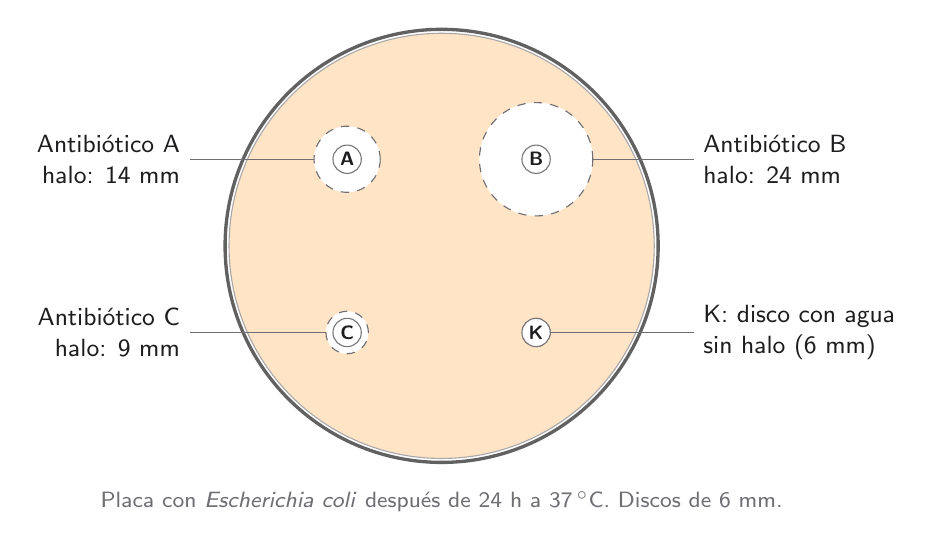
\begin{tikzpicture}[font=\small]
% placa de 90 mm (escala 0,06 cm por mm)
\fill[narc!35] (0,0) circle (2.7);
\draw[tinta!70,very thick] (0,0) circle (2.75);
\draw[gris!60] (0,0) circle (2.7);
% halos (diámetro en mm * 0,03 = radio en cm)
\foreach \p/\r/\l in {{(-1.2,1.1)}/0.42/A,{(1.2,1.1)}/0.72/B,{(-1.2,-1.1)}/0.27/C,{(1.2,-1.1)}/0.18/K}{
  \fill[white] \p circle (\r);
  \draw[gris,dashed] \p circle (\r);
  \fill[white,draw=tinta!60] \p circle (0.18);
  \node[font=\scriptsize\bfseries,text=tinta] at \p {\l};}
\draw[gris] (-1.62,1.1) -- (-3.2,1.1) node[left,text=tinta,align=right] {Antibiótico A\\halo: 14 mm};
\draw[gris] (1.92,1.1) -- (3.2,1.1) node[right,text=tinta,align=left] {Antibiótico B\\halo: 24 mm};
\draw[gris] (-1.47,-1.1) -- (-3.2,-1.1) node[left,text=tinta,align=right] {Antibiótico C\\halo: 9 mm};
\draw[gris] (1.38,-1.1) -- (3.2,-1.1) node[right,text=tinta,align=left] {K: disco con agua\\sin halo (6 mm)};
\node[font=\footnotesize,text=gris,align=center] at (0,-3.25) {Placa con \textit{Escherichia coli} después de 24 h a 37\,$^\circ$C. Discos de 6 mm.};
\end{tikzpicture}
\end{document}
